\documentclass[10pt]{article}
\usepackage[german]{babel}
\usepackage[utf8]{inputenc}
\usepackage{amssymb}
\usepackage{listings}
\usepackage{enumitem}
\usepackage{fancyhdr}
\usepackage{titling}
\usepackage{pgf}
\usepackage{tikz}
\usepackage{array}
\usepackage{ragged2e}
\usepackage{graphicx} 
\usepackage{float}

\usetikzlibrary{arrows,automata}
% \usepackage[latin1]{inputenc}

\title{Informatik 3 Übung - Teil 3\vspace{-2ex}}
\author{Daniel Brun, Michael Hadorn\vspace{-2ex}}

\setlength{\droptitle}{-6em}     % Eliminate the default vertical space
\addtolength{\droptitle}{-4pt}   % Only a guess. Use this for adjustment

\newcolumntype{P}[1]{>{\centering\hspace{0pt}}p{#1}}

\pagestyle{fancy}
% clear any old style settings
\fancyhead{}
\fancyfoot{}

\lhead{ZHAW: Informatik 3}
\rhead{Daniel Brun, Michael Hadorn, Inf 3b}
\fancyfoot[LE,RO]{\thepage}

\usepackage{color}

\begin{document}
\maketitle

% Aufgabe 1  	a: -	b: -
\section*{Aufgabe 1}
Kontrollstrukturen, wie z. B. Schleifen in höheren Programmiersprachen, werden in Maschinensprache über Sprungbefehle realisiert.
\begin{enumerate}[label=\alph*)]
	\item
		\textit{Skizzieren Sie graphisch (schematisch), wie eine For- und eine While-Schleife, die 10-mal \(n \ge 0\) durchlaufen wird, umgesetzt werden könnte. (4 Punkte)}
		\begin{figure}[H]
		  \centering
		     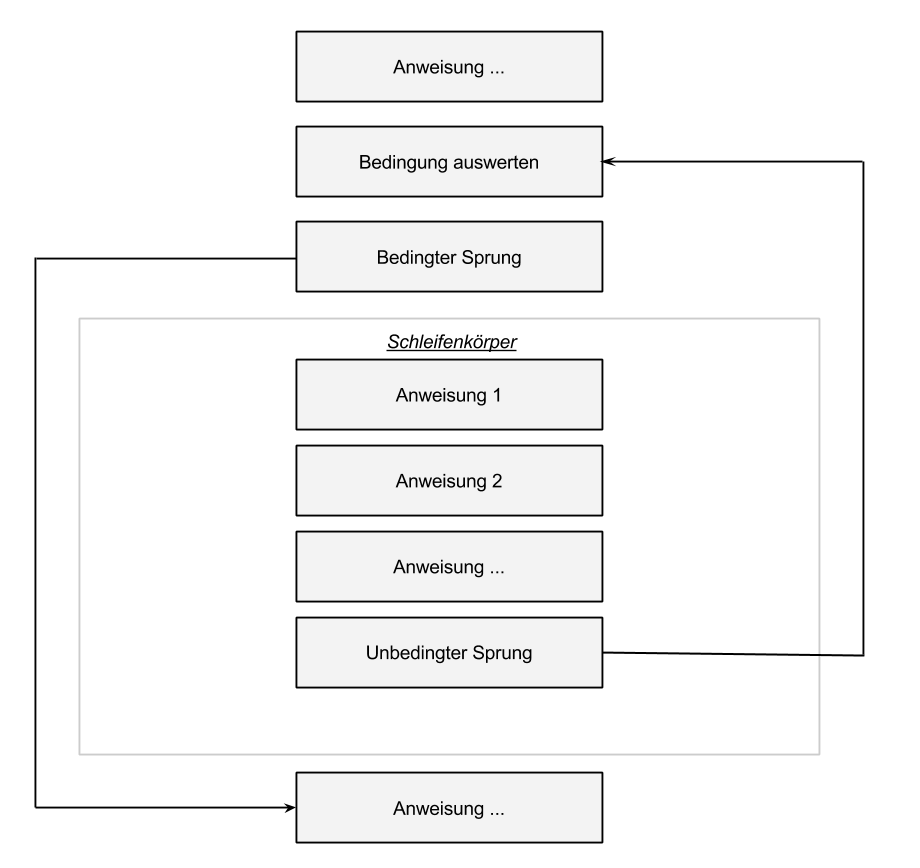
\includegraphics[width=0.7\textwidth]{images/Inf3_S3_1a_1.png}
		  \caption{While-Schleife}
		  \label{fig:Bild1}
		\end{figure}
		%https://docs.google.com/drawings/d/1\_YFmJ5a7F1tx8m\_IIUfy4ascIyVCVj32IRuIXcOcRvA/edit
		%TODO mha: wie genau soll das aussehen? Notation? - Ich begreife nicht wie wir den Counter als while abbilden sollen. Habe mir Skizzen gezeichnet, aber verstehe es nicht...
		%DBRU: Denke es ist so gemeint: https://docs.google.com/drawings/d/1_YFmJ5a7F1tx8m_IIUfy4ascIyVCVj32IRuIXcOcRvA/edit
	
		%TODO mha: Hier ein Entwurf: https://docs.google.com/drawings/d/1G_d7kC5rVWmTCPEIGl2dgUg-T0XShsYCb4RZekhaa88/edit

		\begin{figure}[H]
		  \centering
	     	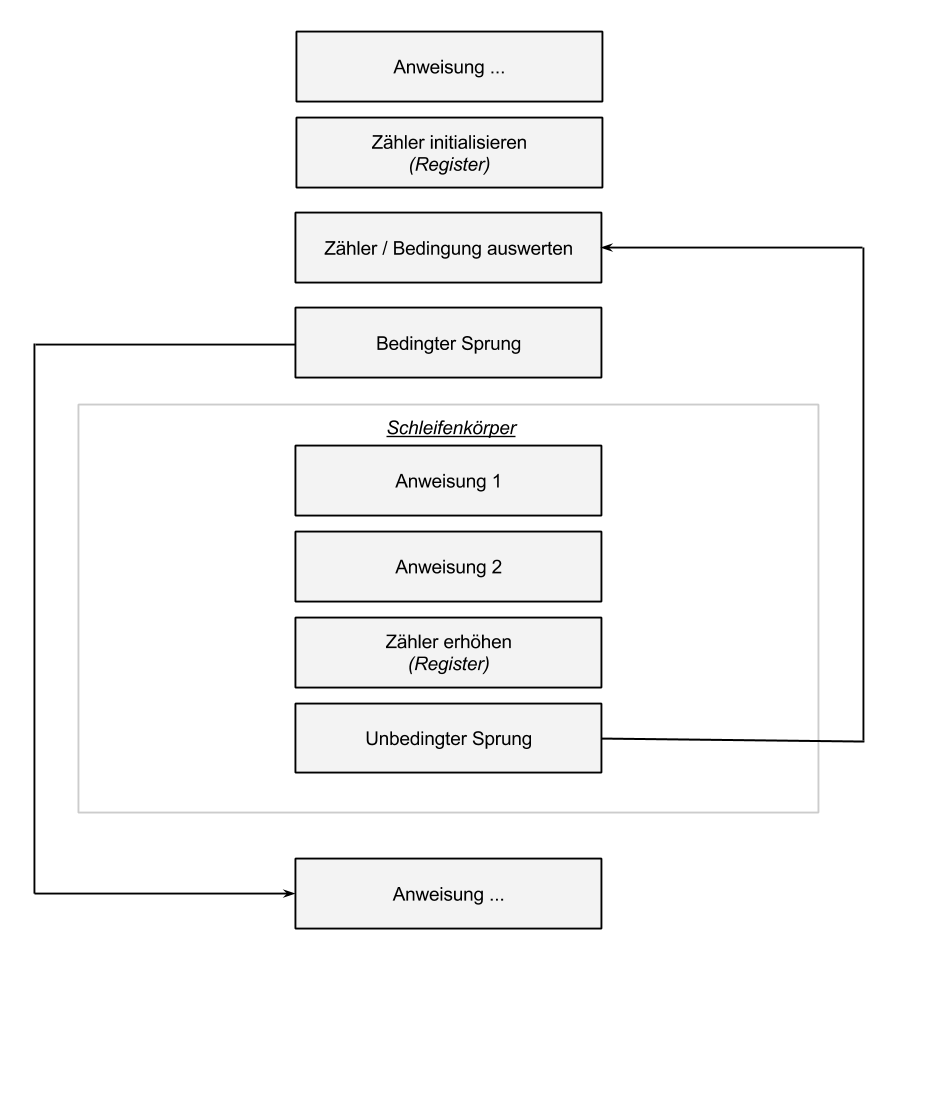
\includegraphics[width=0.7\textwidth]{images/Inf3_S3_1a_2.png}
		  \caption{For-Schleife}
		  \label{fig:Bild2}
		\end{figure}
		%https://docs.google.com/drawings/d/11hUDpEWd6Zmy8Of3nCZrn0jRb9Csq_RhUc_yzb9JpHY/
	\item
		\textit{Mit welcher Einschränkung ist es möglich, die FOR-Schleife mit nur einem Sprungbefehl zu realisieren? Skizzieren Sie auch diesen Fall. (2 Punkte)}
		Wenn sicher ist, dass die Schleife immer mind. einmal durchlaufen wird ("'do-while"') kann die Schleife auch wie folgt realisiert werden:
		%TODO mha: also wie im Beispiel des For's oben (in Aufgabe 1b)?
		%Vorschlag: https://docs.google.com/drawings/d/17wt3-Yg_U2SNcq4RHwBMPir3X0XLH7qGZR3rXht-N_A/edit
		\begin{figure}[H] 
	  		\centering
		     	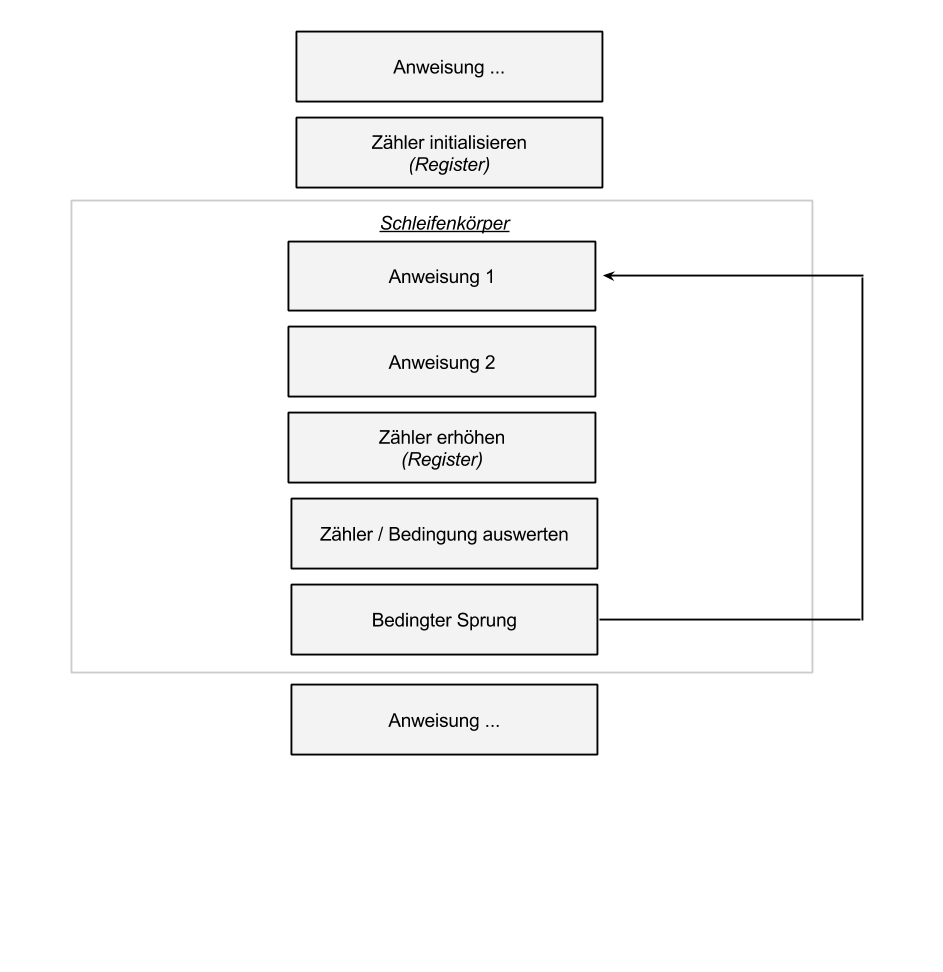
\includegraphics[width=0.7\textwidth]{images/Inf3_S3_1b.png}
	  		\caption{For-Schleife}
	  		\label{fig:Bild3}
		\end{figure}
		
\end{enumerate}


% Aufgabe 2	 	a: OK	b: OK
\section*{Aufgabe 2}
Das Steuerwerk eines Rechners dekodiert die Befehle aus dem OP- Code bzw. dem Maschinencode; für Benutzer sind Befehle mit mnemonische Symbolen leichter zu lesen (und schreiben). Gehen Sie vom Befehlssatz für den "`Mini-Power-PC"' aus.
\begin{enumerate}[label=\alph*)]
	\item
		\textit{Geben Sie für die folgenden Befehle mit mnemonische Symbolen den Maschinencode an: (4 Punkte)}
		
			\begin{tabular}[h]{l l}
				LWDD 1, \#240 & 0100 0100 1111 0000\\
				ADDD \#62 & 1000 0000 0011 1110\\
				Not & 0000 0000 1000 0000\\
				BCD \#15 & 0011 1000 0000 1111\\
			\end{tabular}
	
	\item
		\textit{"'Dekodieren"' Sie die folgenden Befehle in Maschinencode so weit es möglich ist (mnemonische Symbol und Beschreibung): (4 Punkte)}

			\begin{tabular}[h]{l l}
				0001 1111 1110 1111 & BC R3\\
				0101 1010 0000 0000 & LWDD R2, \#512 \\
				0000 1011 0001 1010 & OR R2 \\
				0110 0001 1111 0110 & SWDD Akku, \#502\\ %TODO mha: R0 mit Akku ersetzt, stimmt so oder? DBRU: R0 == AKKU, kommt von daher nicht drauf an ;-)
			\end{tabular}

\end{enumerate}

% Aufgabe 3		 	a: OK	b: OK
\section*{Aufgabe 3}
Der Befehlssatz für den "`Mini-Power-PC"' ist sehr klein / eingeschränkt. Sie haben gelernt, dass Zugriffe auf den Arbeitsspeicher sehr langsam sind (zum Teil deutlich mehr als 100 Zyklen).

\begin{enumerate}[label=\alph*)]
	\item
		\textit{Welchen Befehlstyp würden Sie auf jeden Fall ergänzen, um die Code-Ausführung erheblich zu beschleunigen? Lösung: (3 Punkte)}
		
		Man sollte direkt vom Akku den Wert in ein anderes Register schreiben können und umgekehrt. Sonst muss man diesen Wert immer via Arbeitsspeicher hin und her kopieren.
		
	\item
		\textit{Kann mit dem Befehlssatz ein Arbeitsspeicher von 16 KiB genutzt werden? Antwort bitte begründen. Lösung: (3 Punkte)}
		
		Nein, für die Adressierung stehen jeweils nur 10 Bit zur Verfügung, damit können ohne zusätzliche Komponenten oder einem anderen Aufbau (andere Unterteilung des Arbeitsspeicher) nicht mehr als 1 KiB adressiert werden.
			
\end{enumerate}

\newpage

% Aufgabe 4		 	a: OK	b: -	c: -
\section*{Aufgabe 4}
Gegeben sei der Befehlssatz für den "`Mini-Power-PC"'. Die Aufgabe Summe=a+4*b+8*c soll über ein Programm für den „Mini-Power-PC berechnet werden.

\begin{enumerate}[label=\alph*)]
	\item
		\textit{Schreiben Sie den Programm-Code mit mnemonische Symbolen (in Assembler) (6 Punkte)}
		
		\begin{tabular}[h]{l | l}
			\textbf{Speicher Aufbau} & \textbf{Comment}\\
			\hline
			\#100 = a & Init operation var a\\
			\#102 = b & Init operation var b\\
			\#104 = c & Init operation var c\\
			\#106 = s & Init temp/result var \\
			& \\
			\hline
			\textbf{Befehl} & \textbf{Comment}\\
			\hline
			LWDD R00, \#104 & akku: load var c (to multiplicate with 8)\\
			SLA & value = 2x c \\ %TODO: DBRU SLL oder SLA?, SLA (http://de.wikipedia.org/wiki/Arithmetische_Verschiebung#Arithmetische_Verschiebung)
			SLA & value = 4x c\\
			SLA & value = 8x c\\
			SWDD R00, \#106 & write akku to temp var\\
			& \\
			LWDD R00, \#102 & akku: read var b \\
			SLA & value = 2x b\\
			SLA & value = 4x b\\
			& \\
			LWDD R01, \#100 & r01: load var a\\ %TODO mha: #102 to 100 gewechselt
			ADD R01 & add akku (4xb) and r01 (a)\\
			& \\
			LWDD R01, \#106	 & r01: load temp (8xc) \\
			ADD R01 & add temp to akku \\
			& \\
			SWDD R00, \#106 & write akku to var c -> result\\
			& \\
			END & \\
			
		\end{tabular}

	\item
			\textit{Übersetzen Sie den Code in Maschinencode (4 Punkte)}
			
			01000000 01101000 \\
			00001000 00000000 \\
			00001000 00000000 \\
			00001000 00000000 \\
			01100000 01101010 \\
			\\
			01000000 01100110 \\
			00001000 00000000 \\
			00001000 00000000 \\
			\\
			01000100 01100100 \\ % old 01001000 01100100
			00000111 10000000 \\
			\\
			01000100 01101010 \\ % 01001000 01101010
			00000111 10000000 \\
			\\
			01100000 01101010 \\
			\\
			00000000 00000000
			
%LWDD 0, #504
%SLA
%SLA
%SLA
%SWDD 0, #506
%LWDD 0, #502
%SLA
%SLA
%LWDD 1, #500
%ADD 1
%LWDD 1, #506
%ADD 1
%SWDD 0, #506
%END
			
	\item
			\textit{Berechnen Sie mit Hilfe Ihres Programms: (4 Punkte)}
			Im Bild ist jeweils der Zustand der Register, Akku, Speicher nach der Ausführung des Programmes zu sehen.
			
			
			% ************
			\textit{Summe für a=14, b=7 und c=66}\\
			14 + 4*7 + 8*66 = \textbf{570} (korrekt)
			
			\begin{figure}[H]
				\centering
				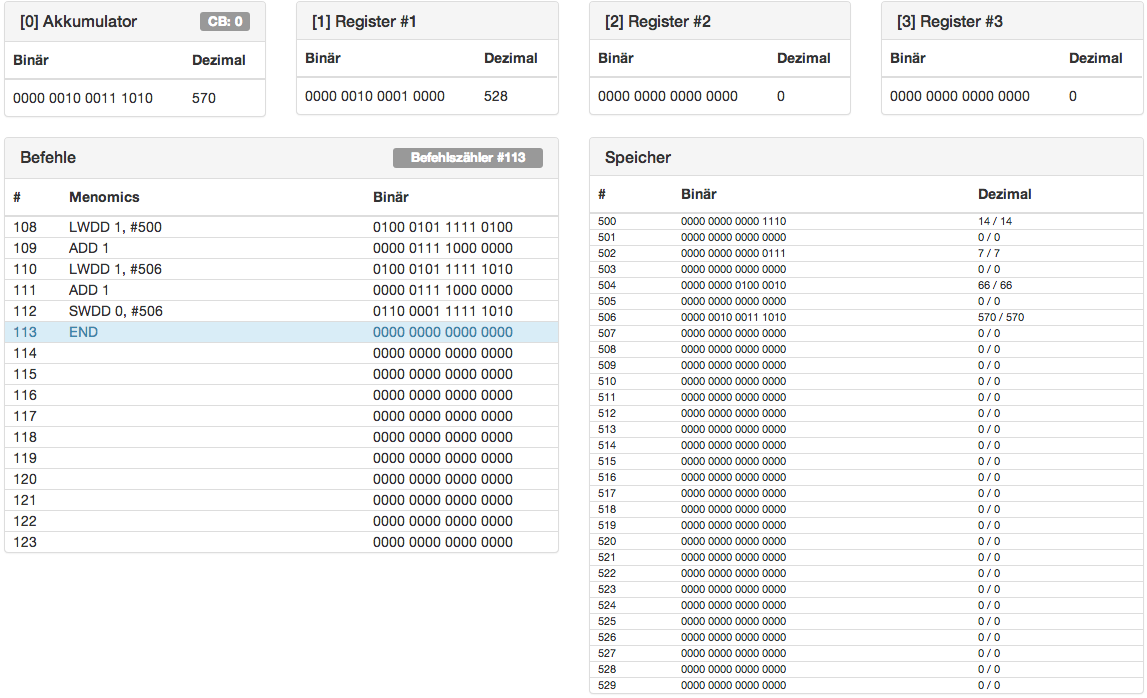
\includegraphics[width=\textwidth]{images/4c_a.png}
				\caption{Mini Power PC Output: 14 + 4*7 + 8*66}
				\label{fig:Bild1}
			\end{figure}


			% ************
			\textit{Summe für a=25, b=-14 und c=-123}\\
			25 + 4*(-14) + 8*(-123) = \textbf{-1015} (korrekt)
			
			\begin{figure}[H]
				\centering
				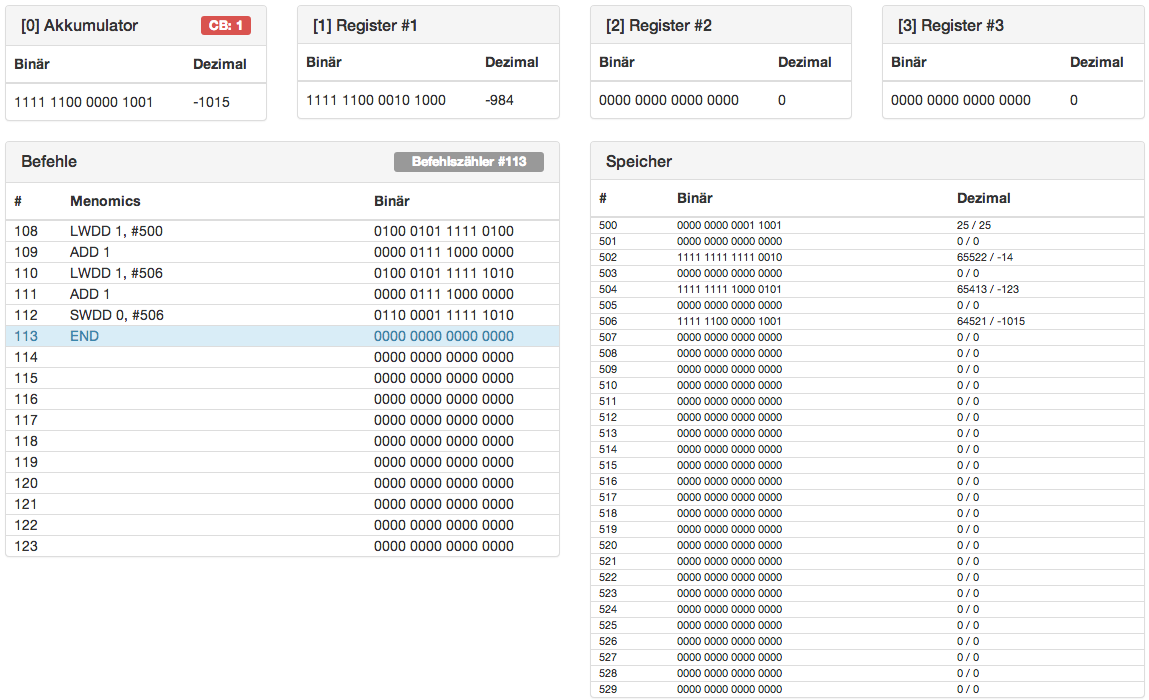
\includegraphics[width=\textwidth]{images/4c_b.png}
				\caption{Mini Power PC Output: 25 + 4*(-14) + 8*(-123)}
				\label{fig:Bild1}
			\end{figure}
			
			
			% ************
			\textit{Summe für a=-125, b=10’000 und c=16}
			
			(-125) + 4*10000 + 8*16 = \textbf{7235}\\
			(stimmt nicht, da overflow beim 4*10000 rechnen)
			
			\begin{figure}[H]
				\centering
				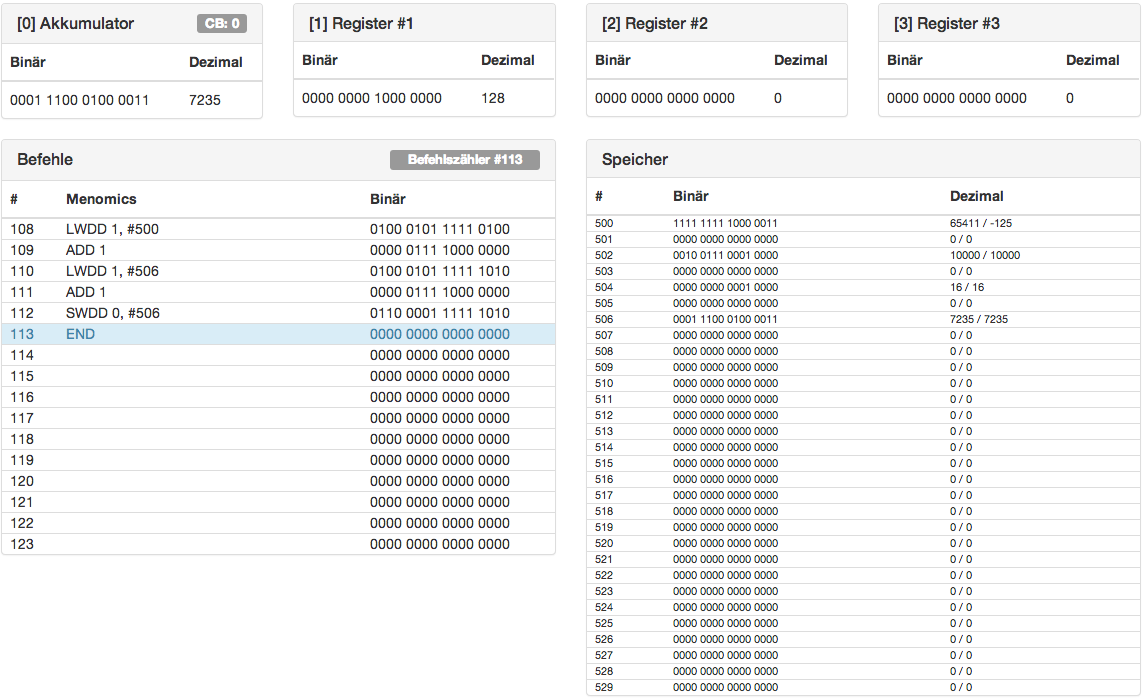
\includegraphics[width=\textwidth]{images/4c_c.png}
				\caption{Mini Power PC Output: (-125) + 4*10000 + 8*16}
				\label{fig:Bild1}
			\end{figure}
			
			
			% ************
			\textit{Summe für a=1000, b=10’000 und c=-2’000}
			
			1000 + 4*10000 + 8*(-2000) = \textbf{-7768}\\
			(stimmt auch hier nicht, da overflow beim 4*10000 rechnen)
			
			\begin{figure}[H]
				\centering
				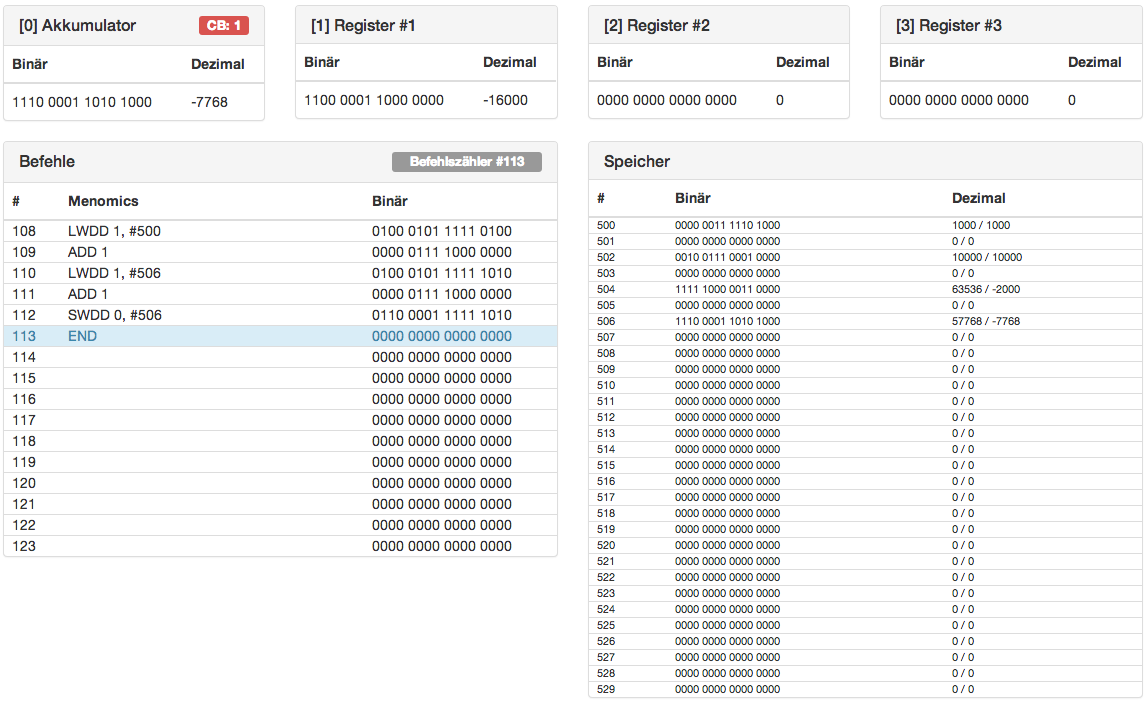
\includegraphics[width=\textwidth]{images/4c_d.png}
				\caption{Mini Power PC Output: 1000 + 4*10000 + 8*(-2000)}
				\label{fig:Bild1}
			\end{figure}
			
			
			%TODO: DBRU: Ist hier einfach das Resultat verlangt oder auch die Zwischenschritte in Binärcode?, Was meinst du?
\end{enumerate}

\end{document}